\def\layersep{1.5cm}

\begin{frame}{What is Deep Learning?}
\begin{minipage}[t]{0.48\linewidth}
\vspace{-0.1cm}
\begin{figure}
	\hspace{-1cm}
	\begin{tikzpicture}[x=1cm, y=1cm, line width=1mm]
    \visible<3-3>{\path [draw=blue,fill=blue!50] (0,0) circle (3.55cm-0.5\pgflinewidth);}
    \visible<2-3>{\path [draw=red,fill=red!50] (0,0) circle (2.4cm-0.5\pgflinewidth);}
    \visible<1-3>{\path [draw=jon_green,fill=jon_green!50,line width=1mm] (0,0) circle (1.15cm-0.5\pgflinewidth);}
    \visible<1-3>{\node[jon_green] at (0,0) {\textbf{DL}};}
    \visible<2-3>{\node[red] at (0,1.65) {\textbf{ML}};}
    \visible<3-3>{\node[blue] at (0,2.9) {\textbf{AI}};}
\end{tikzpicture}
\end{figure}
\end{minipage}
\begin{minipage}[t]{0.48\linewidth}
\visible<1-3>{\textcolor{jon_green}{Deep Learning (DL)} is part of a broader family of \textcolor{red}{Machine Learning (ML)} methods based on artificial Neural Networks. \textit{Wikipedia}}
\vspace{0.2cm}

\visible<2-3>{\textcolor{red}{Machine learning (ML)} is seen as a part of \textcolor{blue}{Artificial Intelligence (AI)} that is devoted to understanding and building methods that \textit{learn}. \textit{Wikipedia}}
\vspace{0.2cm}

\visible<3-3>{\textcolor{blue}{Artificial Intelligence (AI)} is the theory and development of computer systems able to perform tasks that normally require human intelligence, such as visual perception, speech recognition, or decision-making. \textit{Oxford English Dictionary}}
\end{minipage}
\end{frame}


\begin{frame}{Deep Learning Methods}
\textbf{Advantages:}
\vspace{0.4cm}
\begin{itemize}
\item Affordable computational cost (\textit{High offline, low online})
\vspace{0.4cm}
\item Easily parallelizable implementation
\vspace{0.4cm}
\item Great approximation capabilities
\vspace{0.4cm}
\item Exploitable big data
\vspace{0.4cm}
\item Constant advances in computers
\vspace{0.4cm}
\item Trendy among the scientific community
\end{itemize}
\end{frame}


\begin{frame}[t]{Deep Learning Working Areas}
Language Processing
\begin{thebibliography}{1}
\bibitem{DL_lp} \small{D. Otter, J. Medina, and J. Kalita. A Survey of the Usages of Deep Learning for Natural Language Processing. IEEE Transactions on Neural Networks and Learning Systems, 32(2): 604-624, 2021.}
\end{thebibliography}
%https://ieeexplore.ieee.org/abstract/document/9075398?casa_token=un977of__0gAAAAA:f7OQhF6nUr9fNvTePPyrNz2_6Id2GxED9oyu6jtgdhnsaZxykeKdZHdvXJcNp6d0MBlqeY__
\vspace{0.5cm}

Image Processing
\begin{thebibliography}{2}
\bibitem{DL_image} \small{M. Egmont-Petersen, D. de Ridder, and H. Handels. Image processing with neural networks—a review. Pattern Recognition, 35(10): 2279-2301, 2002.}
\end{thebibliography}
%https://www.sciencedirect.com/science/article/abs/pii/S0031320301001789
\vspace{0.5cm}

Healthcare
\begin{thebibliography}{3}
\bibitem{DL_health} \small{A. Esteva et al. A guide to deep learning in healthcare. Nature Medicine, 25: 24–29, 2019.}
\end{thebibliography}
%https://www.nature.com/articles/s41591-018-0316-z?source=post_page---------------------------
\end{frame}


%\begin{frame}[t]{Artificial Neural Networks}
%\visible<1-2>{Artificial neural networks (also known in literature as Neural Networks) are computing systems inspired by the biological neural networks.}
%\vspace{0.3cm}
%
%They are composed of connected units called artificial neurons or nodes. 
%
%\vspace{0.3cm}
%\visible<2>{A node receives signals, then processes them and send the information to neurons connected to it.}
%
%\only<2>{
%\begin{figure}
%	\hspace{-2cm}
%	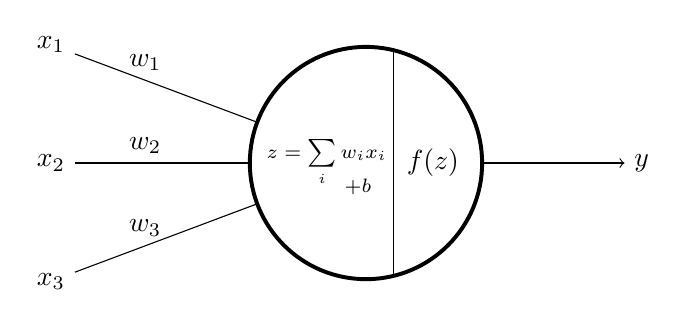
\begin{tikzpicture}
    \node[] at (-4,1.5) (a1) {\textbf{$x_1$}};
    \node[] at (-4,0) (a2) {\textbf{$x_2$}};
    \node[] at (-4,-1.5) (a3) {\textbf{$x_3$}};
    
    \node[] at (0,0) (b) {};
    
    \node[] at (3.5,0) (c) {\textbf{$y$}};  
    
	\path[->] (a1) edge node [near start,above] {$w_1$} (b);
	\path[->] (a2) edge node [near start,above] {$w_2$} (b);
	\path[->] (a3) edge node [near start,above] {$w_3$} (b);
    
    \path[->] (b) edge node [near start,above] {} (c);
    
    \path [draw=black,fill=white,line width=0.5mm] (0,0) circle (1.5cm-0.5\pgflinewidth);
    
%    \node[] at (-0.5,0.6) (b1) {$z$};
%	\node[rotate=90] at (-0.5,0.3) (b1) {$=$};
    \node[] at (-0.5,0) (b1) {{\scriptsize $z=\sum\limits_{i} w_i x_i$}};
    \node[] at (-0.1,-0.3) (b2) {{\scriptsize $ + b$}};
    
    \node[] at (0.35,1.57) (d1) {};
    \node[] at (0.35,-1.57) (d2) {};
    \path[] (d1) edge node [near start,above] {} (d2);
	\node[] at (0.85,0) (b3) {$f(z)$};
\end{tikzpicture}
%\end{figure}
%}
%\end{frame}


\begin{frame}[t]{Artificial Neural Networks}\linespread{1.05}
\vspace{-.2 cm}
\begin{center}
	Approximate: ${\cal I} \approx {\cal I}_{\phi} := A_k \circ N \circ A_{k-1}  \circ \cdots \circ N \circ A_1 $\\
\end{center}
\only<1-2>{
	\vspace{0.2 cm}
	\centerline{$N$ -- Non-linear activation function  \hspace{0.3 cm};\hspace{0.3 cm} $A_k$ -- Affine transformation}
	\vspace{0.6cm}
\begin{figure}
	\vspace*{-0.25in}
	\begin{tikzpicture}
	\visible<2>{
	\node[] () at (0,-0.2) {\begin{tikzpicture}[scale=0.62]
		\begin{axis}[
		%ticks=none,
		height=0.5\textwidth,
		width=0.1\textwidth,
		scale only axis,
		enlargelimits=false,
		axis on top,
		xlabel={Resistivity [$\Omega$m]},
		xtick={0,1.2,2.39},
		xticklabels={100,200,300},
		ytick={0.93,1.85,2.78,3.7,4.65,5.56,6.50,7.44,8.37,9.305,10.24,11.18,12.08,13},
		yticklabels={130,120,110,100,90,80,70,60,50,40,30,20,10,0},
		ylabel={Deep [m]},
		label style={font=\tiny},
		tick label style={font=\tiny}] 
		\addplot[thick] graphics[xmin=0,xmax=3,ymin=0,ymax=13] {Diapos/Intro/Figures/resis1};
		\end{axis}
		\end{tikzpicture}};
		}
		
	\node[] () at (4.3,0.2) {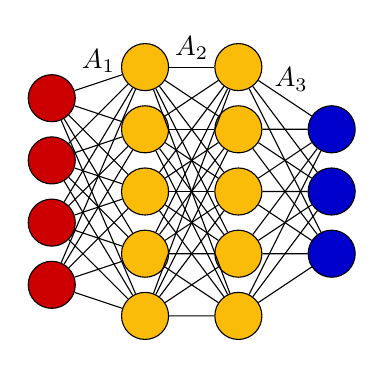
\begin{tikzpicture}[scale=0.79]
		\tikzstyle{every pin edge}=[<-,shorten <=1pt]
		\tikzstyle{neuron}=[circle,fill=black!25,minimum size=17pt,inner sep=0pt]
		\tikzstyle{input neuron}=[neuron,draw=black,fill=red!80!black];
		\tikzstyle{output neuron}=[neuron,draw=black,fill=blue!80!black];
		\tikzstyle{hidden neuron}=[neuron,draw=black,fill=yellow!50!orange];
		\tikzstyle{annot} = [text width=4em, text centered]
			
			% Draw the input layer nodes
		\foreach \name / \y in {1,...,4}
		% This is the same as writing \foreach \name / \y in {1/1,2/2,3/3,4/4}
		\node[input neuron] (I-\name) at (0,-\y) {};
			
			% Draw the hidden layer nodes
		\foreach \name / \y in {1,...,5}
		\path[yshift=0.5cm]
		node[hidden neuron] (H-\name) at (\layersep,-\y cm) {};
			
			% Draw the hidden layer nodes
		\foreach \name / \y in {1,...,5}
		\path[yshift=0.5cm]
		node[hidden neuron] (H2-\name) at (\layersep+\layersep,-\y cm) {};
			
			
			% Draw the output layer node
		\foreach \name / \y in {1,...,3}
		\path[yshift=-0.5cm]
		node[output neuron] (O-\name) at (\layersep+\layersep+\layersep,-\y cm) {};
			
			% Connect every node in the input layer with every node in the
			% hidden layer.
		\foreach \source in {1,...,4}
		\foreach \dest in {1,...,5}
		\path (I-\source) edge (H-\dest);
			
		\foreach \source in {1,...,5}
		\foreach \dest in {1,...,5}
		\path (H-\source) edge (H2-\dest);
			
			% Connect every node in the hidden layer with the output layer
		\foreach \source in {1,...,5}
		\foreach \dest in {1,...,3}
		\path (H2-\source) edge (O-\dest);

	    \node[] () at (0.75, -.4) {$A_1$};	
		\node[] () at (2.25, -0.2) {$A_2$};
		\node[] () at (3.85,-.7) {$A_3$};
			% Annotate the layers
		\end{tikzpicture}};
	\node[] () at (4.3, 2.8) {Neural Network};		
	\visible<2>{	
	\node[] () at (8.8, 1.2) {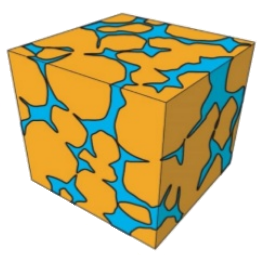
\includegraphics[width=2.5cm]{Diapos/Intro/Figures/res1}};
	\node[] () at (8.8,-1.4) {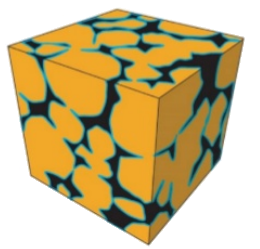
\includegraphics[width=2.5cm]{Diapos/Intro/Figures/res2}};
	\node[] () at (8.4, 2.8) {Output};
	\node[] () at (0.2, 2.8) {Input};
		
	\draw [decorate,very thick,decoration={brace,amplitude=10pt},xshift=-4pt,yshift=0pt]
		(1.3,2.8) -- (1.3,-2.4);
	\draw [decorate,very thick,decoration={brace,amplitude=10pt},xshift=-4pt,yshift=0pt]
		(7.5,-2.4) -- (7.5,2.8);
		
	\node[right] () at (9.0, 0.0) {\scriptsize Water};		
	\node[right] () at (9.0, -2.5) {\scriptsize Oil};	
	}			
\end{tikzpicture}
\end{figure}}
\only<3>{
	\vspace{0.4cm}
	
	$A_k$ -- Affine transformation: \hspace{0.1cm} $A_k \cdot x+b_k$
	\vspace{0.4cm}
	
	$N$ -- Non-linear activation function:

	\begin{figure}
	\centering
		\begin{subfigure}{.5\textwidth}
		\centering
		\begin{tikzpicture}[scale=0.7]
\begin{axis}[
    xmin=-2.5, xmax=2.5,
    ymin=-1.5, ymax=1.5,
    axis lines=center,
    axis on top=true,
    domain=-2.5:2.5,
    ylabel=$tanh(x)$,
    xlabel=$x$,
    x label style={at={(axis description cs:0.5,-0.1)},anchor=north},
    y label style={at={(axis description cs:-0.1,.5)},rotate=90,anchor=south},
    ]

    \addplot [mark=none,draw=blue,ultra thick] {tanh(\x)};
%    \node [right, red] at (axis cs: 1,0.7) {$y = \tanh x$};
    
    %% Add the asymptotes
%    \draw [blue, dotted, thick] (axis cs:-2.5,-1)-- (axis cs:0,-1);
%    \draw [blue, dotted, thick] (axis cs:+2.5,+1)-- (axis cs:0,+1);
\end{axis}
\end{tikzpicture}

		%	\caption{Tanh}
		\label{fig:tanh}
		\end{subfigure}%
		\begin{subfigure}{.5\textwidth}
		\centering
		\begin{tikzpicture}[scale=0.7,
  declare function={
    func(\x)= (\x < 0) * (0)   +
                   + (\x >= 0) * (\x);
  }
]
\begin{axis}[
    xmin=-2.5, xmax=2.5,
    ymin=-1.5, ymax=1.5,
    axis lines=center,
    axis on top=true,
    domain=-2.5:2.5,
  ylabel=$ReLU(x)$,
  xlabel=$x$,
     x label style={at={(axis description cs:0.5,-0.1)},anchor=north},
    y label style={at={(axis description cs:-0.1,.5)},rotate=90,anchor=south}, % added
]

\addplot [blue,ultra thick] {func(x)};
\end{axis}
\end{tikzpicture} 
		%	\caption{Tanh}
		\label{fig:tanh}
		\end{subfigure}
%	\caption{A figure with two subfigures}
	\label{fig:test}
	\end{figure}
	}
\end{frame}


\begin{frame}[t]{Deep Learning in Geophysics}
%They train a CNN to approximate the inverse operator. They use different metrics to control the value of the loss and use dropout method as regularization. 
%\begin{thebibliography}{4}
%\bibitem{geo_1} \small{D. Moghadas. One-dimensional deep learning inversion of electromagnetic induction data using convolutional neural network. Geophysical Journal International, 222(1): 247-259, 2020.}
%\end{thebibliography}
%https://academic.oup.com/gji/article-abstract/222/1/247/5818323
They train a CNN to approximate the inverse operator. They use the data misfit loss function with MSE metric and add a regularization term.
\begin{thebibliography}{5}
\bibitem{geo_2} \small{B. Liu et al. Deep Learning Inversion of Electrical Resistivity Data. IEEE Transactions on Geoscience and Remote Sensing, 58(8): 5715-5728, 2020.}
\end{thebibliography}
\vspace{0.2cm}

The model outputs several likely inverse solutions and it also predicts their probabilities. 
\begin{thebibliography}{5}
\bibitem{geo_2} \small{ S. Alyaev and A. H. Elsheikh. Direct multi-modal inversion of geophysical logs using deep learning. Earth and Space Science, 9, e2021EA002186, 2022.}
\end{thebibliography}
%https://ieeexplore.ieee.org/abstract/document/8994191?casa_token=dBQ0UUmOSyUAAAAA:vre7sUUy3QZ6OyaCxwigpHbmfR-HZdQWcXJ-Z0YMwDyMWXFnPISVJuEJlslqWLvuSZ1pvHa-iGvy
\vspace{0.2cm}

%En este utiliza un loss normal, el missfit, pero parte de una solucion a priori (o puede ser random tambien). Ellos no entrenan el inverso aqui, lo evaluan en el loss.
%\begin{thebibliography}{6}
%\bibitem{geo_3} \small{Y. Shi, X. Wu, and S. Fomel. Deep learning parameterization for geophysical inverse problems. SEG Global Meeting Abstracts, 36-40, 2020.}
%\end{thebibliography}
%%https://library.seg.org/doi/abs/10.1190/iwmg2019_09.1

\visible<2>{In the first part of this dissertation, \textbf{we analyze the behavior of different loss functions while solving inverse problems using Deep Learning.}
\begin{thebibliography}{6}
\bibitem{DL_me} \small{M. Shahriari, D. Pardo, J. A. Rivera et al. Error control and loss functions for the deep learning inversion of borehole resistivity measurements. International Journal for Numerical Methods in Engineering, 122(6): 1629-1657, 2021.}
\end{thebibliography}}
\end{frame}